\documentclass{article}

% Packages
\usepackage{titling}
\usepackage[utf8]{inputenc}
\usepackage[english]{babel}
\usepackage{amsmath,amssymb}
\usepackage{graphicx}
\usepackage{float}
\usepackage{subcaption}
\usepackage[hidelinks]{hyperref}
\usepackage{xcolor}
\usepackage{listings}
\usepackage[a4paper, margin=1in]{geometry}
\usepackage{multicol}
\usepackage{booktabs}
\usepackage{array}
\usepackage{geometry}% Package for margin adjusting
\usepackage{titlesec} % Package to change title format
\usepackage{enumerate}
\usepackage{enumitem}




\graphicspath{{Figures/}}

\geometry{
  left=2cm, % adjust the left margin
  right=2cm, % adjust the right margin
  top=2cm, % adjust the top margin
  bottom=2cm, % adjust the bottom margin
}



%%%%%%%%%%%%%%%%%%%%%%%%%%%%%%%%%%%%%%%%%%%%%%%%%%%%%%%%%%%%%%

%First page structure:
% - Pretitle (unipv logo)
% - Title (Course, Project title)
% - Author info (name, course, contacts)
% - Date

\pretitle{
  \begin{center}
    \vspace{-1.5cm}
  \LARGE
  
\includegraphics[width=15.1cm,height=3.05cm]{Logo_unipv.png}\vspace*{0.6cm}\\[\bigskipamount]
}
\posttitle{\end{center}}

\title{\Large Digital Content Retrieval Course\vspace{0.3cm}\\
    \rule{\textwidth}{0.6pt}\vspace{0.3cm}\\
    \textbf{Video Curriculum: Who am I ?}\vspace{0.1cm}\\
    \rule{\textwidth}{0.6pt}\vspace{0.2cm}}

\author{Andrea Alberti\vspace{0.2cm}\\
    \small Computer Engineering - Data Science\\
    \small University of Pavia, Italy \\
    \small Email: andrea.alberti01@universitadipavia.it\vspace{0.2cm}\\
    \small Video Curriculum link: \url{https://youtu.be/n3CD9vUCMOc}}

\date{ April 21, 2023}

%%%%%%%%%%%%%%%%%%%%%%%%%%%%%%%%%%%%%%%%%%%%%%%%%%%%%%%%%%%%%%

%Start document

\begin{document}

\begin{titlepage}
    
    \maketitle %insert pretitle, title and author defined above
    \thispagestyle{empty} %remove page number
    \begin{multicols*}{2}
        \hrule
        \tableofcontents %insert index
        \vspace{3cm}
        \newcolumn
        \hrule
        \begin{abstract}
            \noindent
            \\
            This project is about the creation of a video curriculum to be used in job seeking. The goal was that of making a dynamic and engaging video that presents individual skills, knowledge and
            other information that a classic paper CV cannot communicate. Lots of multimedia data objects (images, texts and music) were used and merged together with animations and transitions using
            a professional video editing software \textit{'Wondershare Filmora 12'}.
            Project management tools and methodologies were employed to ensure the project was completed on time and with all the required contents. The project considers a thorough evaluation of privacy and copyright concerns to ensure adherence to legal and ethical standards. 
            Additionally, the project facilitated the acquisition of novel proficiencies in video editing and compression methodologies. To ensure access to the video without falling in reproduction
            and distribution issues, it was uploaded on the popular streaming platform \textit{'YouTube'} and can be accessed using the following link: \url{https://youtu.be/n3CD9vUCMOc}.\\
            \\
            \begin{center} \textbf{Keywords}\\\end{center}Video Curriculum • Video Editing • Project Management • SWOT • GANTT • WBS • Risk Analysis

        \end{abstract}

    \end{multicols*}
  
\end{titlepage}


\newpage

\pagenumbering{arabic}

%%%%%%%%%%%%%%%%%%%%%%%%%%%%%%%%%%%%%%%%%%%%%%%%%%%%%%%%%%%%%%

%document structure definition

\begin{multicols}{2}
    

\section{Introduction}
The primary objective of this project is to develop a video curriculum that effectively showcases my qualifications to prospective employers. The project was 
executed with a strong focus on professionalism, leveraging project management tools to ensure a high-quality outcome.
The concept involves creating a dynamic video comprising a series of concise videos enriched with relevant text and images, each highlighting a different 
facet of my professional profile. These videos were seamlessly combined using transitions and effects, utilizing the capabilities of a professional video 
editing software like Wondershare Filmora 12.
The final product is uploaded to a popular video sharing platform, YouTube, but will only be accessible with my explicit permission. This approach ensures 
that the video remains securely shared with targeted employers and maintains its intended professional context.

\section{Project Management}
To ensure a professional approach to project execution, a range of project management tools were used for planning, executing, and controlling the project.
The employed tools are: Work Breakdown Structure (WBS), Gantt Chart, SWOT Analysis, and Risk Analysis. Each of them plays a crucial role in guiding the project's 
progress and mitigating potential challenges. A brief overview of each tool is provided in the following sections.

    \subsection{Work Breakdown Structure}
    The WBS is a hierarchical and timeless decomposition of the project into smaller and more manageable tasks. It is used to facilitate project planning and it is the first project management
    tool to be faced. The WBS I used in shown in figure \ref{fig:wbs}.

        

    \noindent
    The WBS structure comprises multiple layers, each representing a distinct level of detail. 
    \begin{figure}[H]
        \centering
        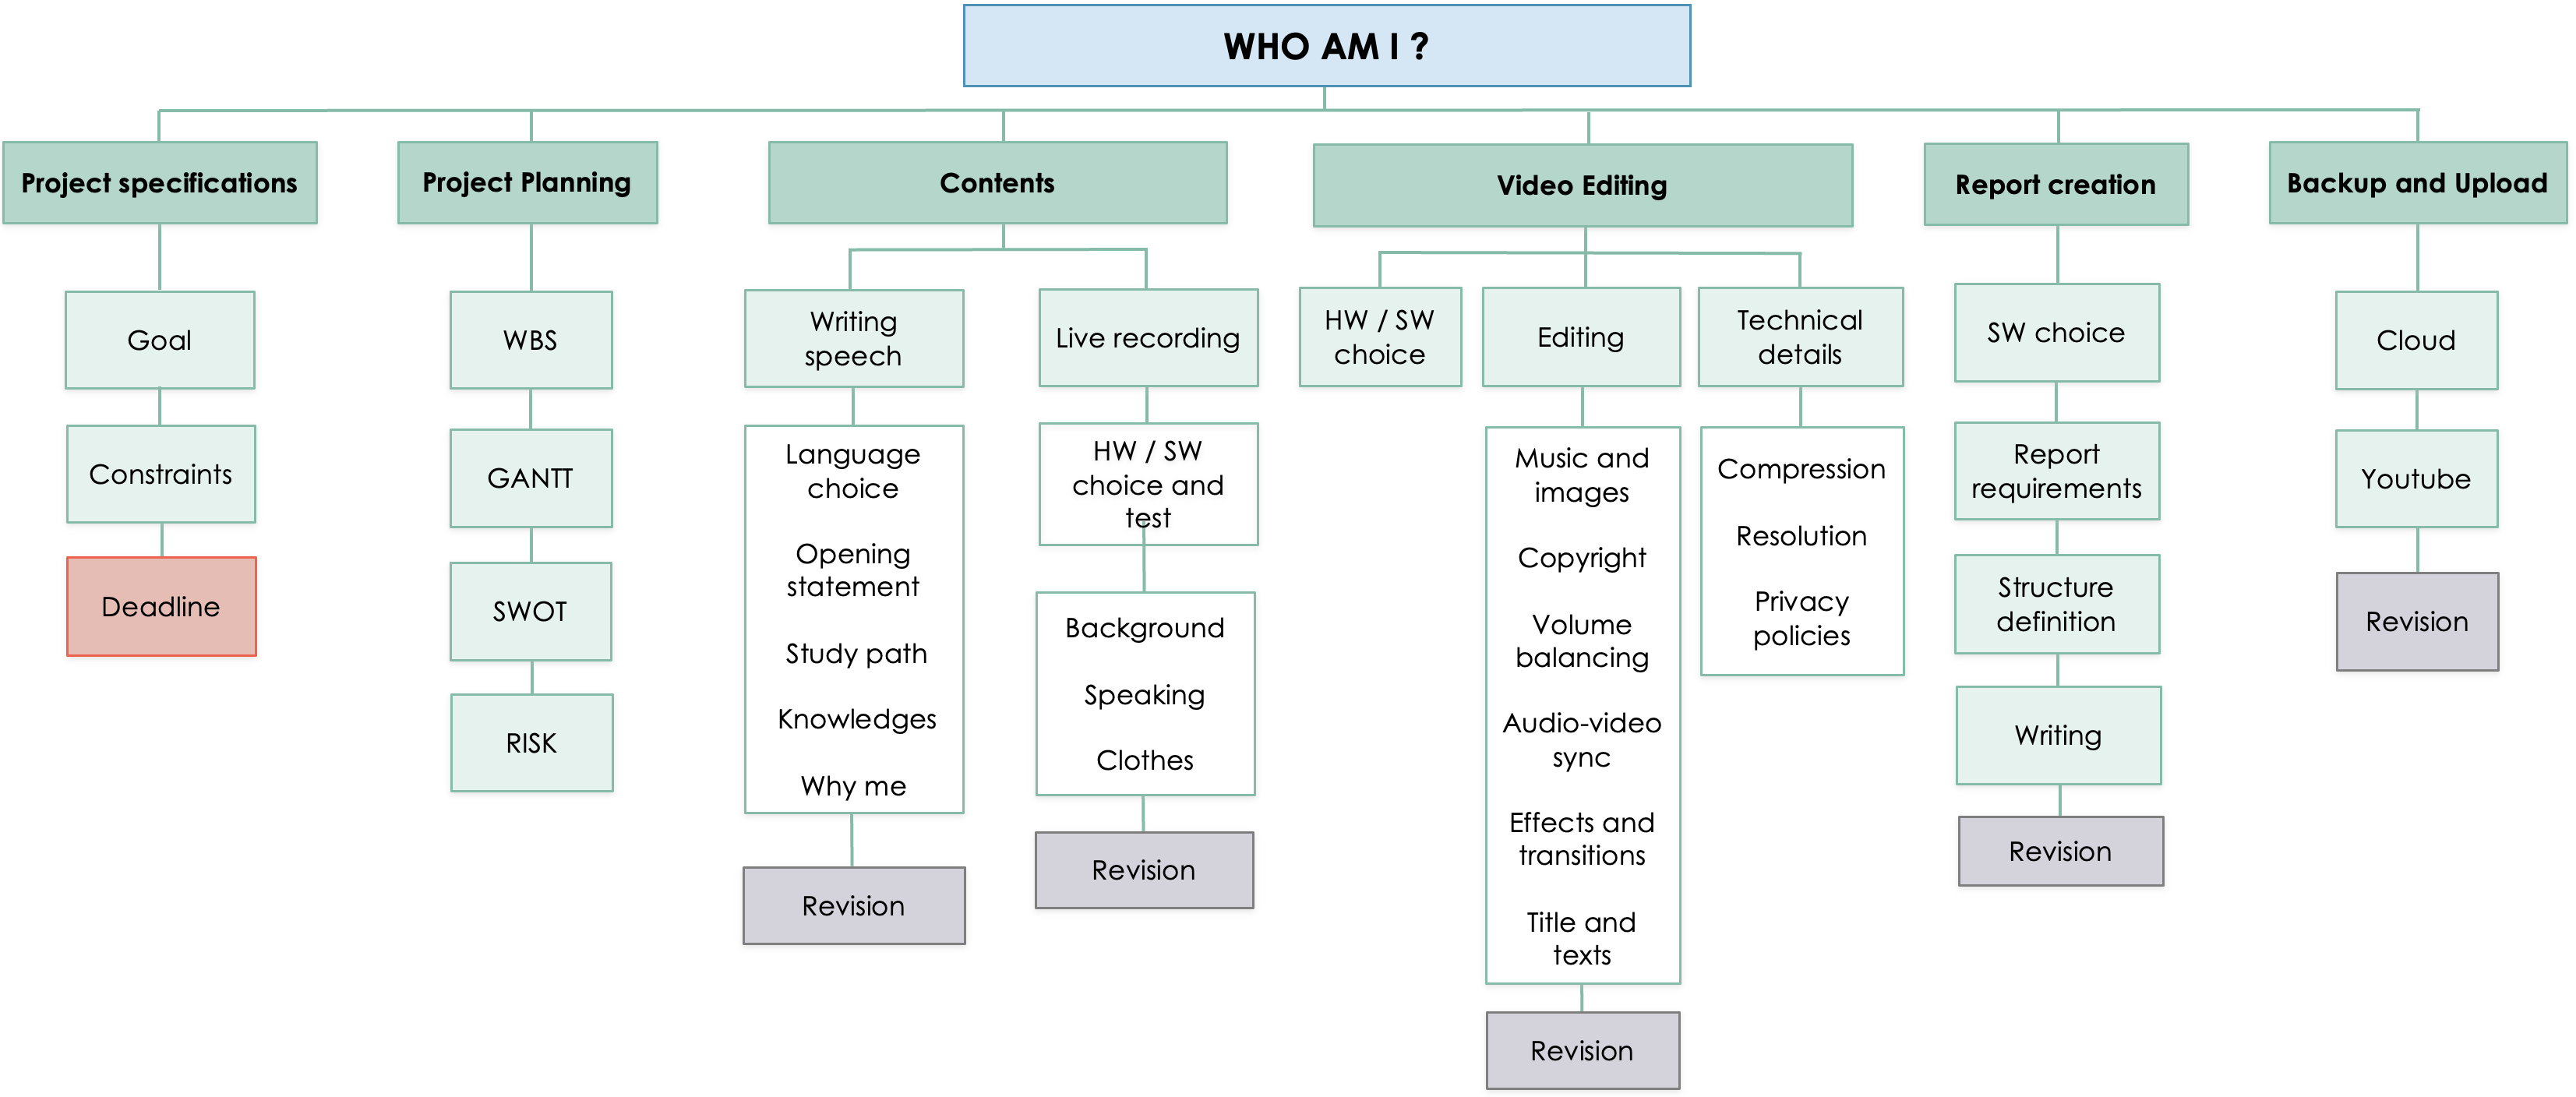
\includegraphics[width=0.96\textwidth]{WBS.png}
        \caption{Work Breakdown Structure}
        \label{fig:wbs}
    \end{figure}
    
    The first layer encompasses the entire project itself, 
    while the second layer consists of the main tasks to be accomplished.  
    This hierarchical decomposition continues further, with each subtask being further broken down into smaller tasks.
    The colors used in the structure are not arbitrary; they serve as visual indicators of specific information. The green color signifies a task itself, 
    while the white color contains important content or information related to the parent task. For instance, when examining the "Writing speech" task, the 
    white square below it contains the sections that must be included in the speech. The red color is used to highlight critical information, while light 
    purple is employed to draw attention to essential operations, such as the revision process. This latter follows all tasks involving 
    content production and includes activities like grammar check or others, depending on the father task.
    To address potential ambiguities or unclear tasks, detailed explanations are provided below for better understanding and clarity.
    
    \begin{itemize}[leftmargin=*]
    \item Constraints: are the limitations that the project must respect. For example the video must elapse in no more than three minutes.
    \item Opening statement: is a catchy phrase that introduces the video, different from the classic repetitive introductions.
    \item Copyright: refers to the permission of using the multimedia data objects inserted in the video.
    \item Report requirements: are the contents that must be included in the report.
    \item Compression: select a proper codec video that balances video quality and memory usage.
    \item Resolution: pick a good tradeoff between video quality and bandwidth required to see fluently the video.
    \item Cloud: refers to the way the backup is done. In this case a private cloud is used.
    \end{itemize}
    \clearpage

    \subsection{GANTT Chart}
    The GANTT Chart is a graphical representation of the project schedule and it is used to control the project execution. It is a bar chart that shows the tasks to be done, the start and end date
    so that the timing of the project can be easily visualized. The contents are basically the same of the WBS, but in this case chronological information is present.
    The GANTT Chart I used is shown in figure \ref{fig:gantt}.

    \noindent
    The structure and the title are those used in the WBS. The main tasks are visually represented by dark grey rows and are displayed in bold font, while the 
    subtasks are represented by light grey rows. Each subtask is accompanied by its start date and the allocated number of days for completion.
    
    Within each row, the timing representation is provided on the right side, where colored cells correspond to the number of days required for the task. The 
    colors hold specific meanings, as indicated in the legend at the top of the figure. Each color represents a different risk status based on the completion 
    percentage and the remaining days. Green indicates that the task is on track, cyan signifies a slight delay, blue suggests
    \begin{figure}[H]
        \centering
        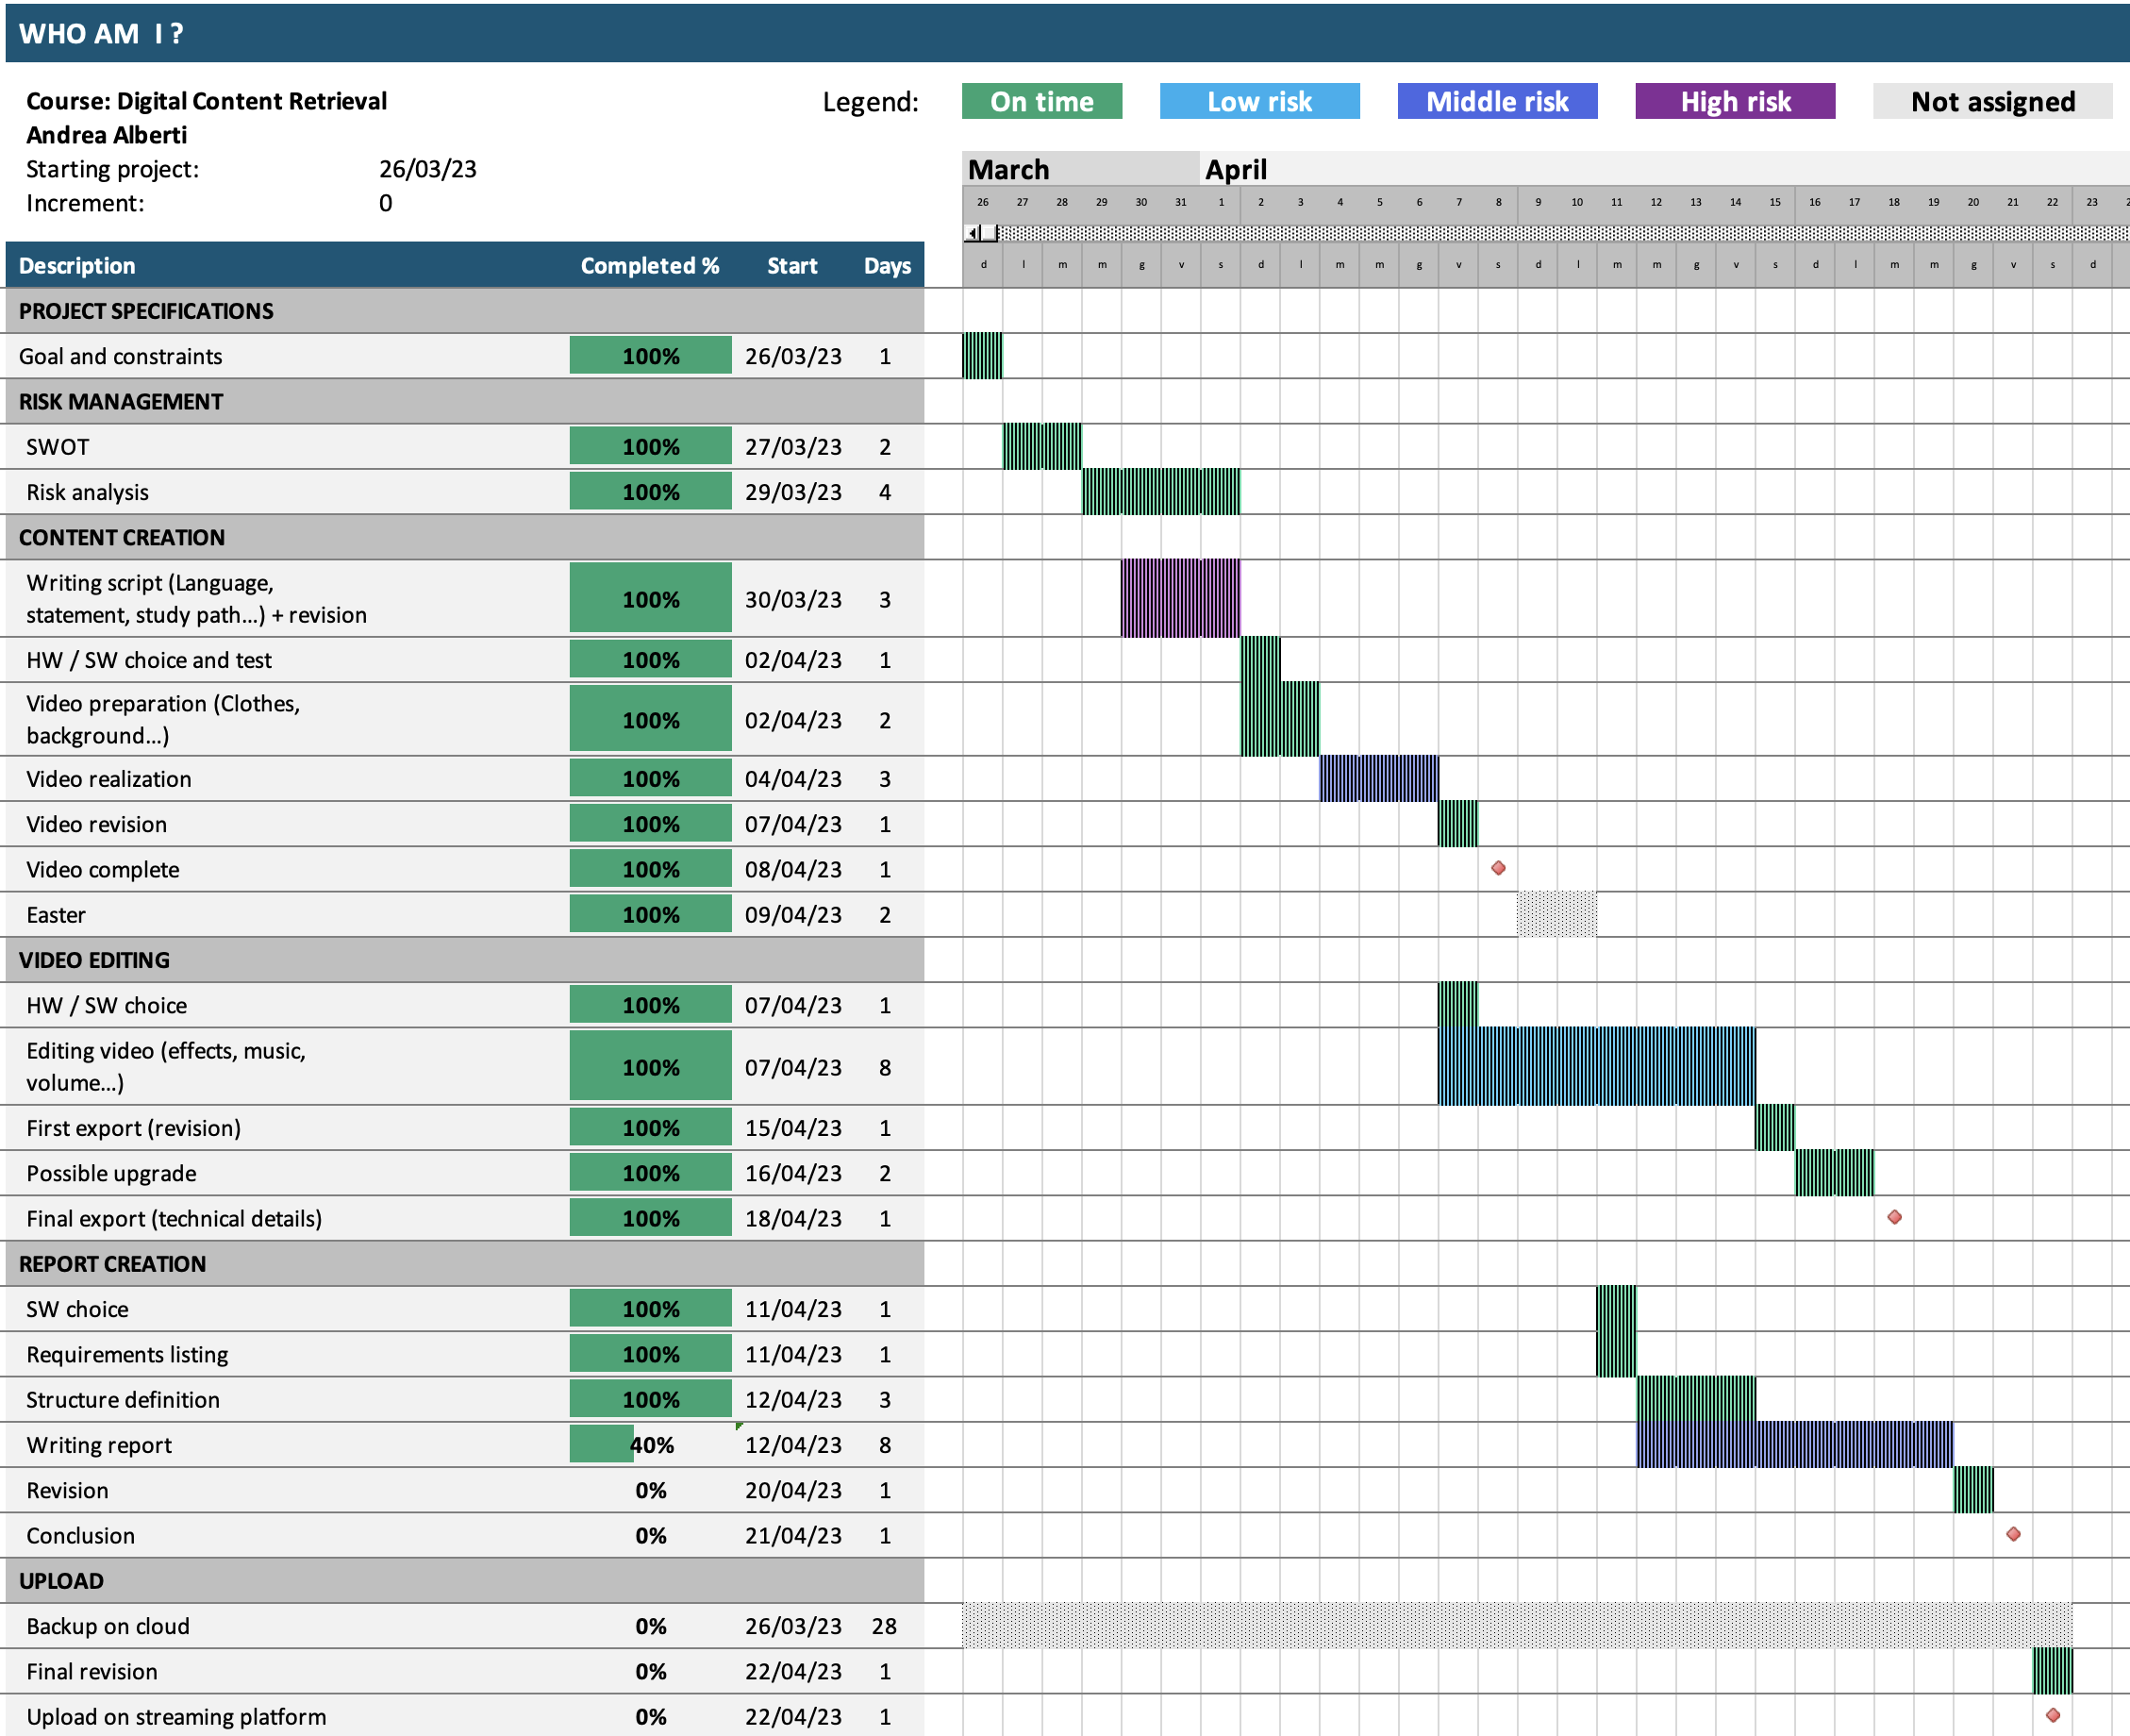
\includegraphics[width=1\textwidth]{GANTT.png}
        \caption{GANTT Chart}
        \label{fig:gantt}
    \end{figure}
    \noindent
    \\
    \\
    a moderate delay that requires 
    attention, and purple indicates a significant delay demanding immediate focus to meet the deadline.

    It is evident that certain tasks posed a risk of not being completed on time, such as the "Writing script" task that required numerous changes and adjustments. 
    Consequently, additional effort was invested to ensure its timely completion. The use of colors facilitated tracking the progress, ensuring that all completed 
    tasks were finished on schedule.

    The red dots signify milestones, representing crucial tasks with specific deadlines. The red vertical lines indicate the present day when this section of the 
    report is being written. As the report creation is experiencing some delay, its timing is color-coded as blue.
    
    The remaining tasks are currently on schedule, given that there are still a few days left to complete them.

   

    \clearpage
    \subsection{SWOT Analysis}
    SWOT stays for Strengths, Weaknesses, Opportunities and Threats. It is a tool used to analyze the project and its environment. It facilitates the identification 
    of the reasons why a project should be done (Opportunities), the reasons why it shouldn't be done (Weaknesses) and the things we can count on in making
    the project (Strengths). 
    Additionally, it allows to identify potential challenges that could impact the project implementation (Threats). 
    The SWOT analysis I conducted is presented in Figure \ref{fig:swot}.

   
    This project presents numerous opportunities and a limited number of weaknesses. The opportunities include the potential for personal growth through learning new skills 
    and the possibility to distinguish myself from the vast pool of job seekers. Additionally, as a student, the project carries the added benefit of contributing towards the 
    achievement of 12 exam credits.

    On the other hand, the main weaknesses revolve around my limited experience in video editing and filming. However, these weaknesses provide an opportunity to acquire 
    valuable skills in the domain of multimedia production and enhance my expertise.

    There are also some threats and it is crucial to
    \begin{figure}[H]
        \centering
        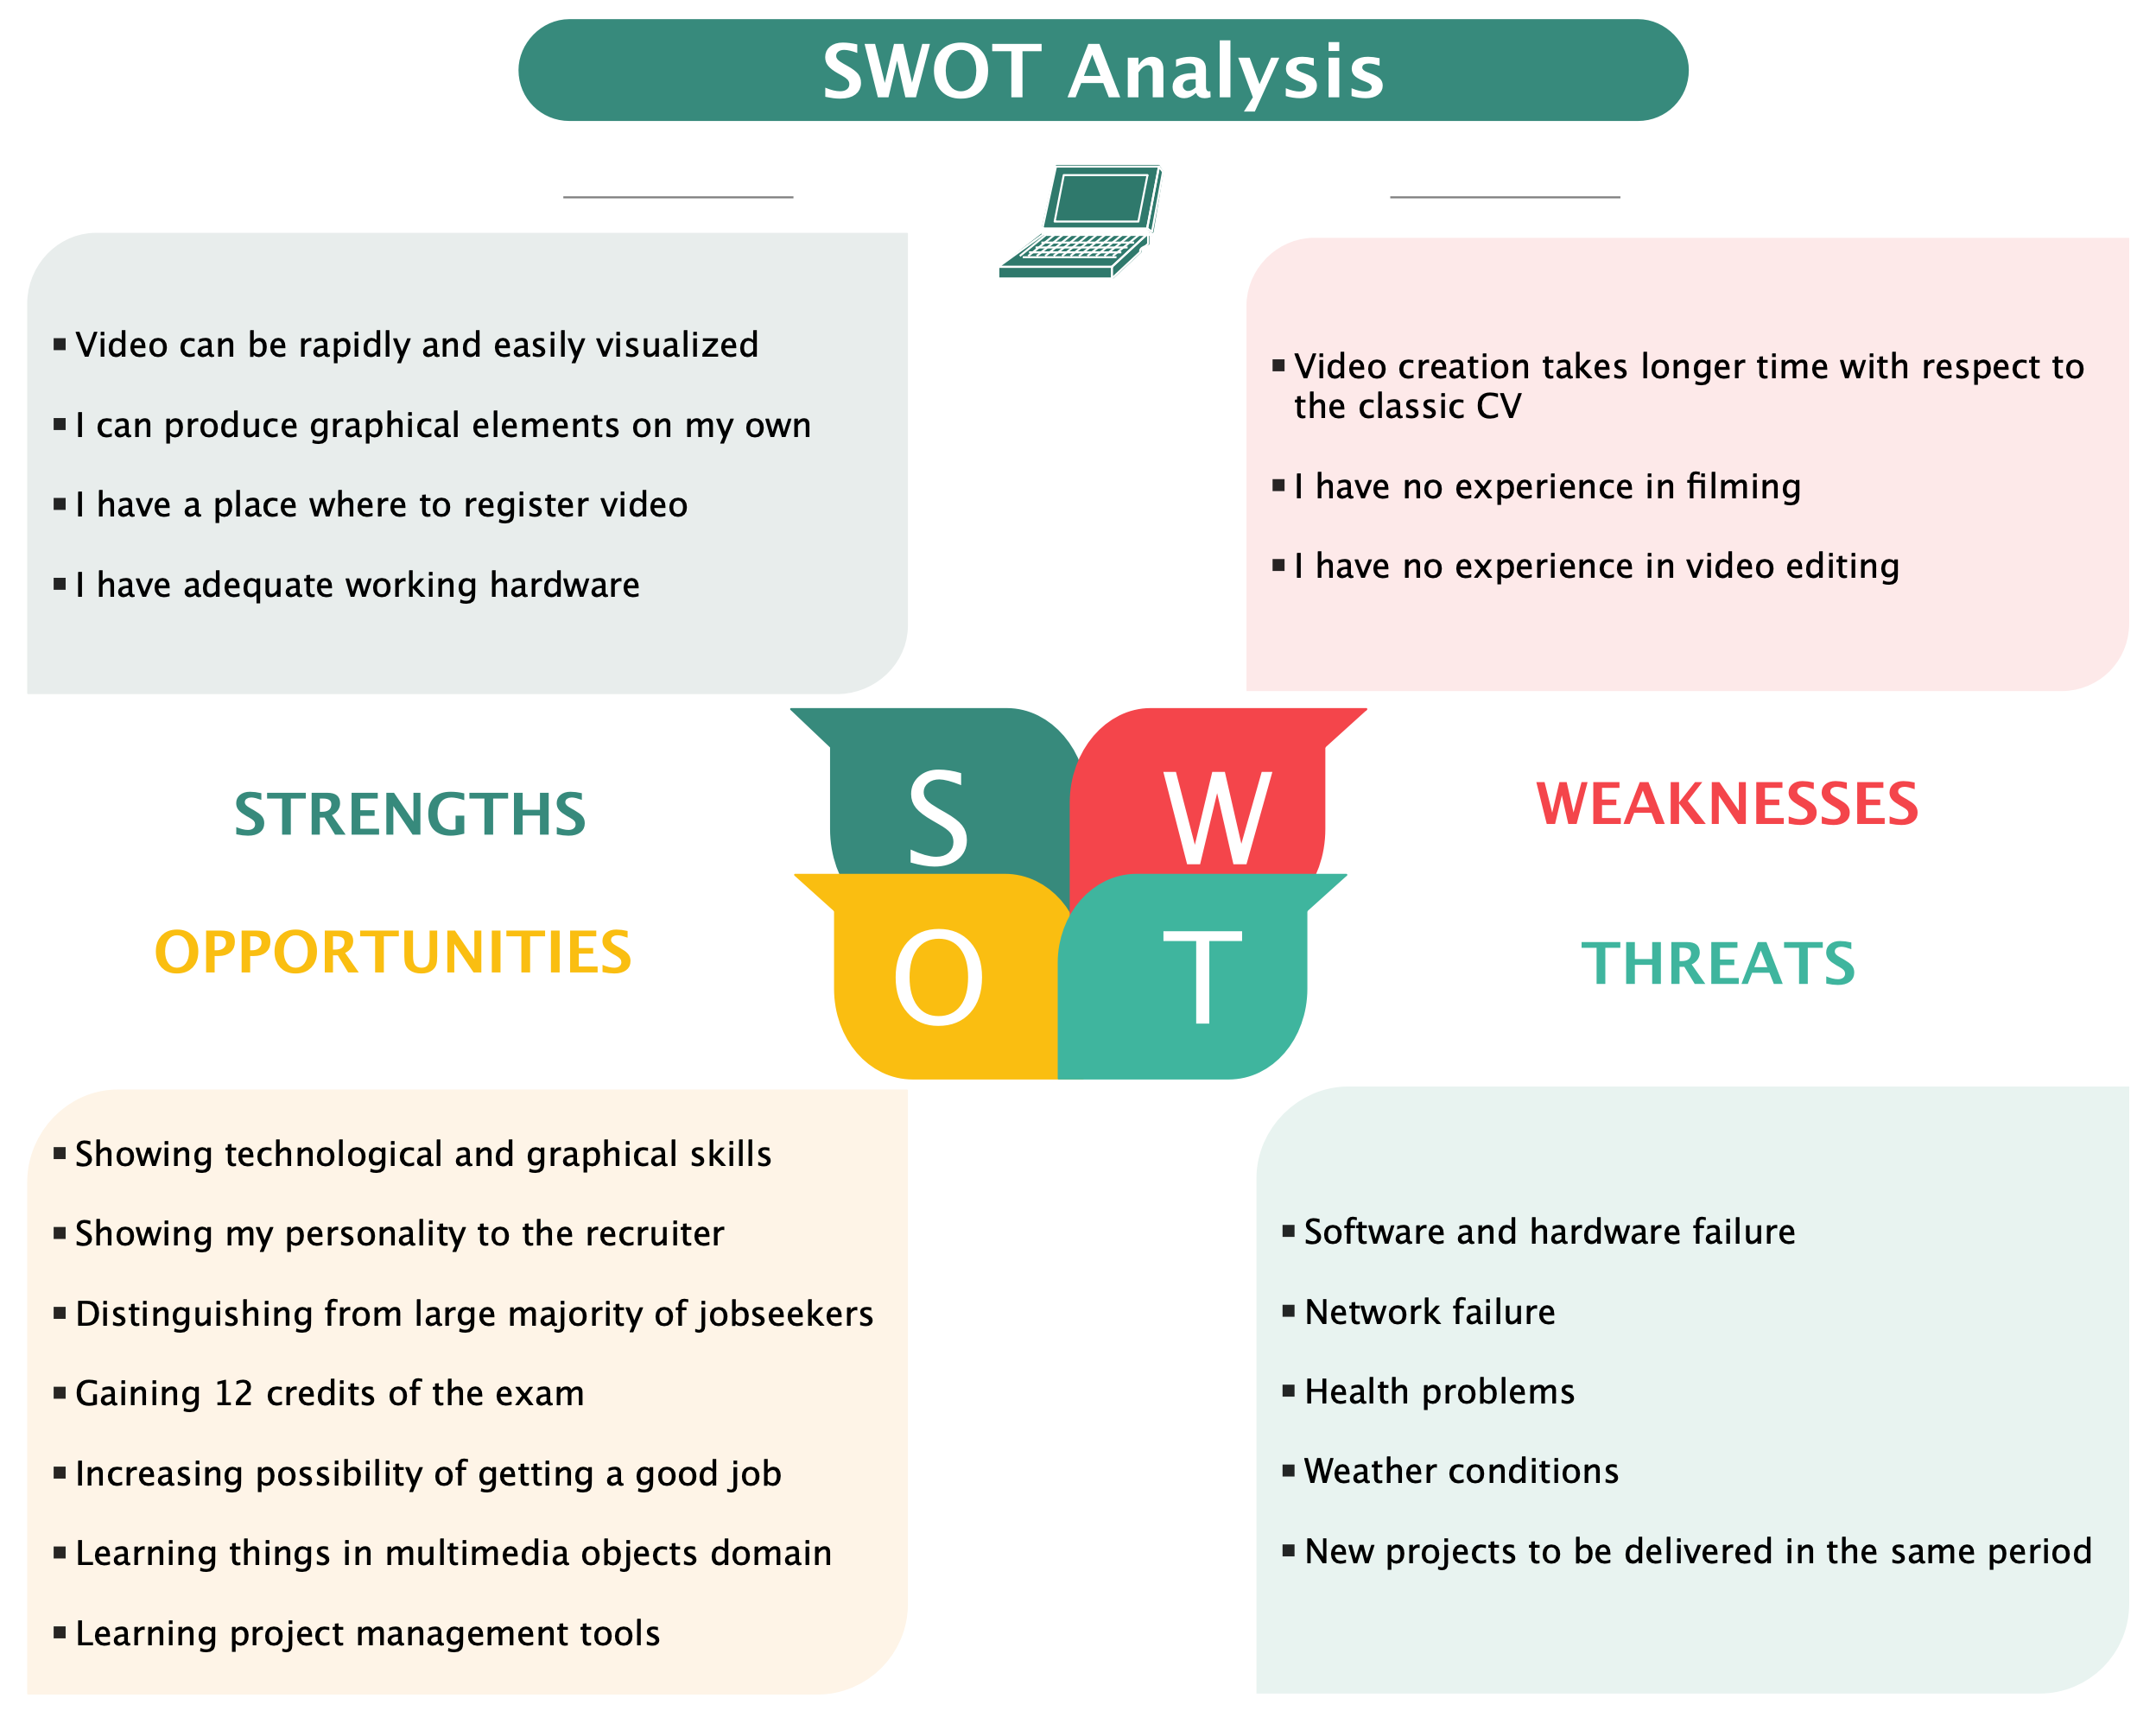
\includegraphics[width=1\textwidth]{SWOT.png}
        \caption{SWOT Analysis}
        \label{fig:swot}
    \end{figure}

    \noindent
    consider them in the risk analysis, establishing countermeasures to try avoiding surprises during the project execution.

    \subsection{RISK Analysis}
    Risk analysis is a valuable tool used to identify potential risks that may impact the project. These risks are classified based on their potential impact and the 
    likelihood of occurrence. By categorizing risks, appropriate actions can be established to effectively address them.

    The concept of risk encompasses both positive and negative aspects. Negative risks are those that pose a threat to the project and require proactive measures to 
    either avoid or mitigate them, especially when they carry significant impact. On the other hand, positive risks stem from opportunities and can bring potential 
    benefits to the project. For these risks, the recommended course of action is to capitalize on them and maximize their advantages.

    The risk analysis I conducted is depicted in figure \ref{fig:risk_pos} and figure \ref{fig:risk_neg}.\\
    \noindent
    The risks have been documented in the rows, each accompanied by an assessment of its impact and probability of occurrence. Both impact and probability are 
    categorized into three levels: low, medium, and high. \\
    \clearpage

    In the case of network failure risks, no specific measures have been implemented due to their infrequent 
    occurrence and the low impact they would have on the project, as network connectivity is only required during the upload phase. Since the project execution is 
    primarily offline, with local NAS backups, network failures are unlikely to disrupt the project.

    For positive risks, where no actions have been defined, it is because these risks are seen just as opportunities to be exploited. It is worth noting 
    that the risk analysis has influenced the project's GANTT chart. For instance, to address the risk of new projects being delivered within the same timeframe, 
    the project deadline was moved forward by one week.


        \begin{figure}[H]
            \centering
            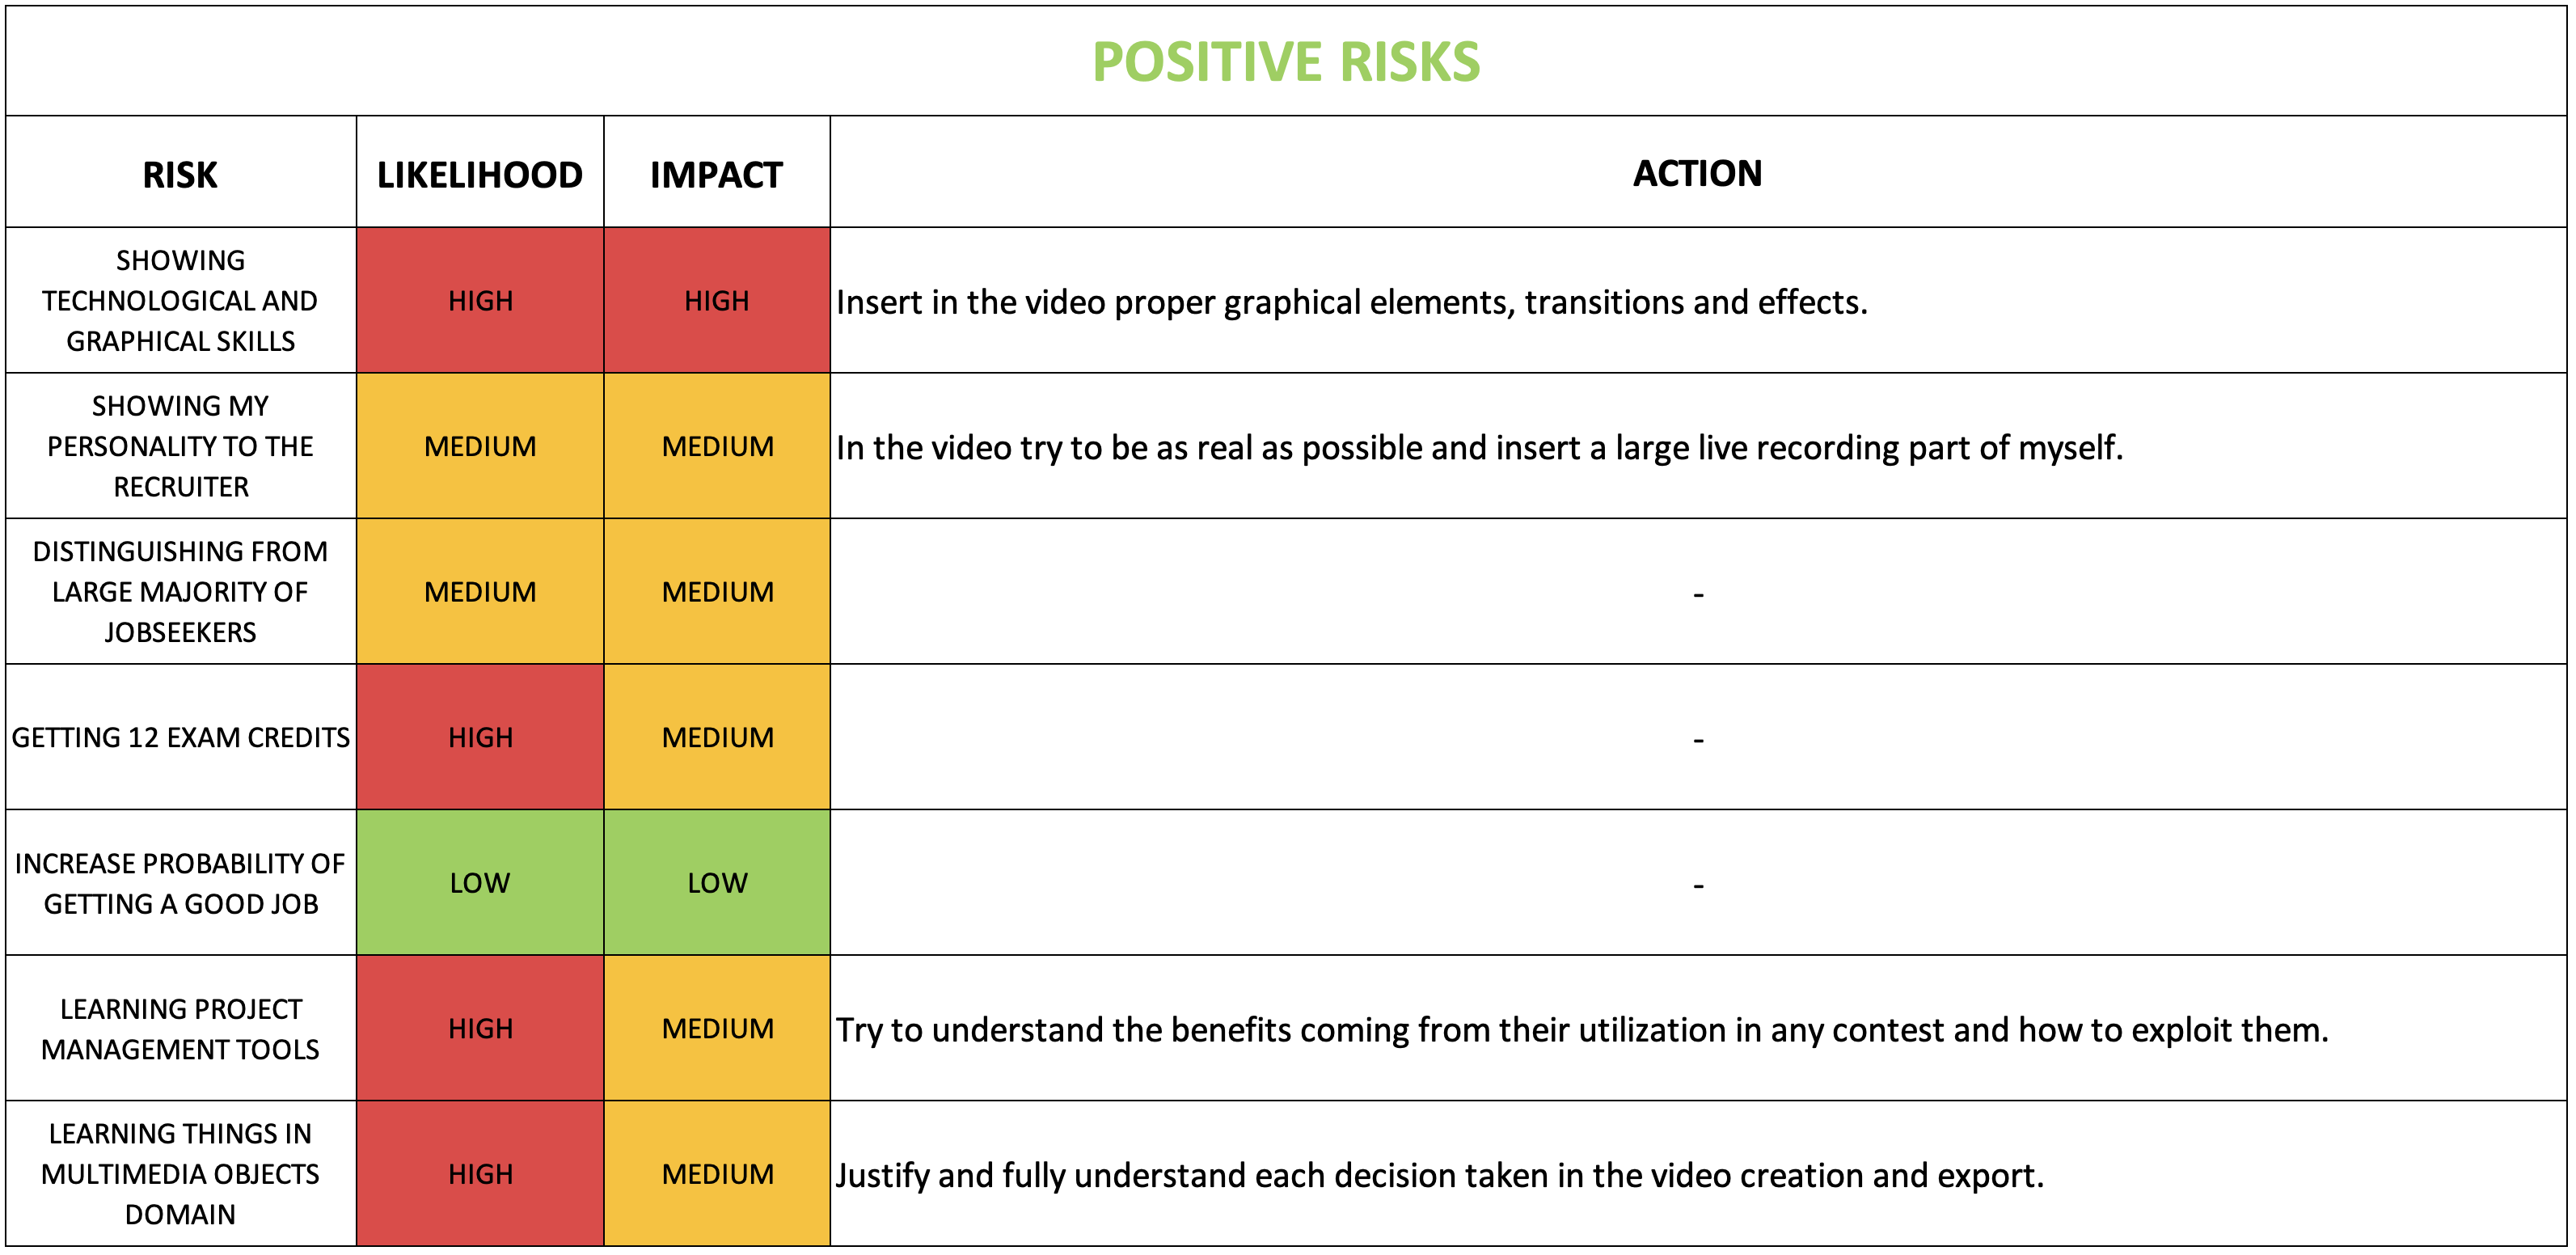
\includegraphics[width=1\textwidth]{POSITIVE RISK.png}
            \caption{POSITIVE RISK Analysis}
            \label{fig:risk_pos}
        \end{figure}

        \vspace{-0.1cm}

        \begin{figure}[H]
            \centering
            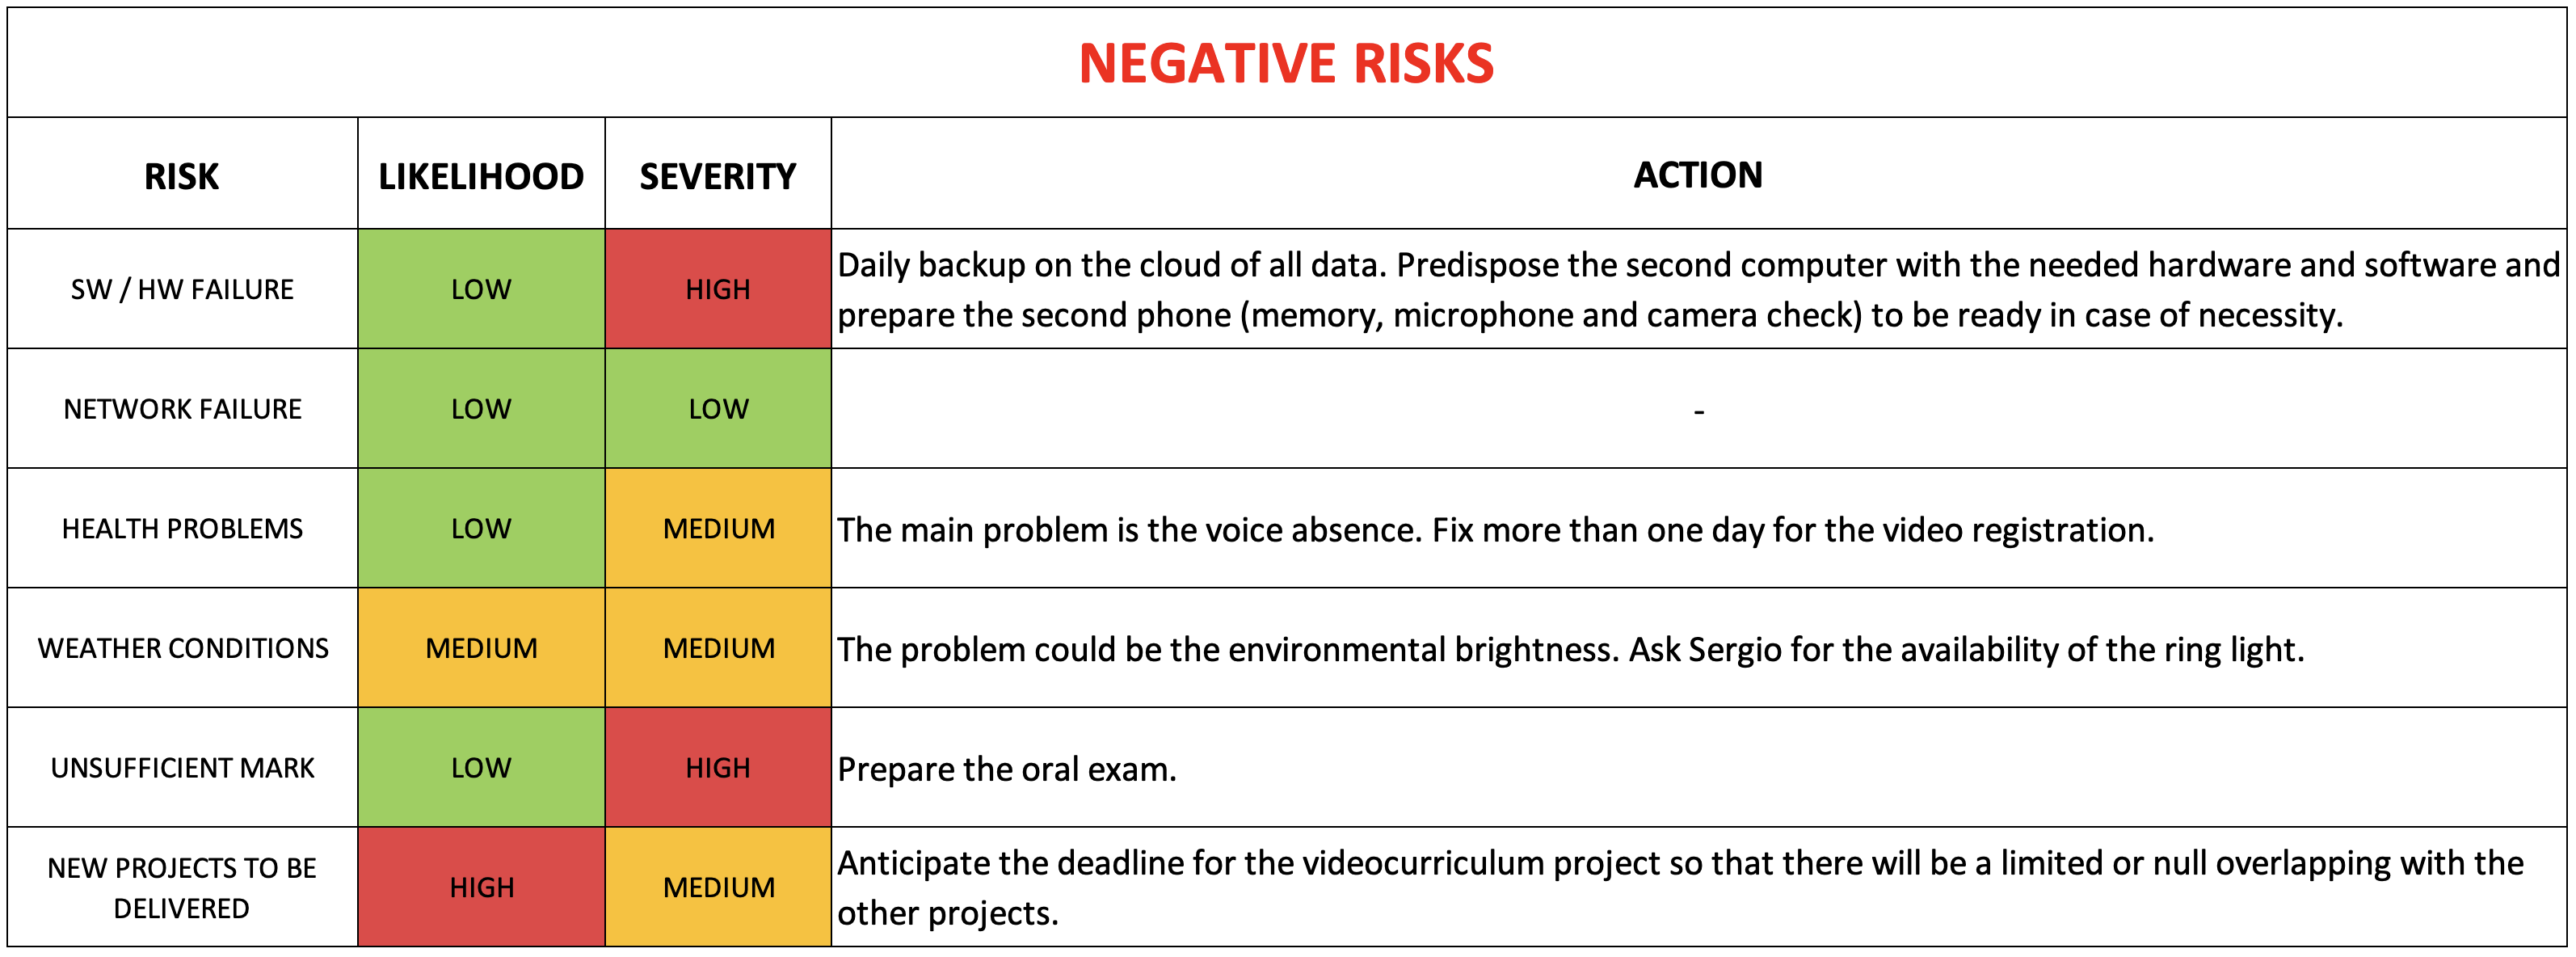
\includegraphics[width=1\textwidth]{NEGATIVE RISK.png}
            \caption{NEGATIVE RISK Analysis}
            \label{fig:risk_neg}
        \end{figure}

        
    \noindent

\section{Project Execution}
The video curriculum creation required the execution of several tasks, the most demanding ones were the content creation and the video editing. To successfully complete the two tasks lots of challenges
had to be faced and all of them, together with the solutions adopted, are described in this section.

    \subsection{Content Creation}
    The content creation is the most important part of the project. It is the phase in which the script is written and the multimedia objects are created. 
    \clearpage
    \noindent
    The script, together with the live recording 
    are the core of the video curriculum and their quality heavily affects the final result.

    
        \subsubsection{Writing Speech}
        The objective was to create a script different from the conventional format, effectively conveying information to the viewer that goes beyond what is typically 
        found in a traditional written CV. In addition to showcasing my skills, projects, and academic achievements, it was essential to allow my personality to emerge.

        To achieve this, I devised an impactful opening statement in the script that demonstrated my determination and ambition to attain my goals. The script proceeded by weaving 
        a narrative, connecting various pieces of information in a logical manner. The conclusion of the speech tells to the viewer what I can offer and why I am the right 
        choice.

        Italian was selected as the language for the video, considering the target audience. However, there are plans to create an English version in the future to reach a wider 
        audience.

        \subsubsection{Live Recording}
        The objective was to present the written speech in a dynamic manner, incorporating frequent changes in camera angles and the inclusion of multimedia elements. To achieve this, 
        the recording process was divided into multiple shots, each captured from different camera angles, and subsequently merged during the video editing phase. Each segment was 
        recorded multiple times to ensure the selection of the best footage. However, a challenge arose regarding the need for consistent background and even lighting across the various shots.

        To address this issue, a green screen was utilized in conjunction with a ring light, which provided uniform illumination and served as a recording support. The hardware used for 
        capturing the video, along with its specifications, are outlined in Table \ref{tab:recording_hardware}. The decision to employ high-quality equipment was motivated by the intention 
        of creating videos that could potentially be utilized for other purposes in the future. In this phase, the HEIF format was favored over JPEG/H.264 due to its efficiency.

            \begin{table}[H]
                \centering
                \caption{Recording Hardware}
                \label{tab:recording_hardware}
                \begin{tabular}{|c|c|c|c|c|}
                    \hline
                    \textbf{Device} & \textbf{Resolution} & \textbf{Format}\\ \hline
                    iPhone 13 & 4K, 60 fps, HDR & HEIF / HEVC \\ \hline

                    
                \end{tabular}    
            \end{table}


    \subsection{Video Editing}
    The goal of the video editing was that of making a dynamic video that could capture the attention of the viewer. Therefore, images, videos, music and texts were used together with frequent changes of camera angle.
    Aspects about copyright are treated in the \textit{'Multimedia Data Objects'} section.

        \subsubsection{Tools}
        The main problem faced was the lack of experience in video editing. To solve it, a prior research on the video editing software was done, to choose the best compromise between ease of use and features.
        The final choice was \textit{'Wondershare Filmora 12'}. The images were adapted to match with the video in timing and position and animations were added to increase fluidity and avoid abrupt changes as
        much as possible. The text was used to graphically show information like the skills, avoiding listings in the speech and engaging the viewer.
        The different videos shot were merged using proper transitions and the music was added to the background, balancing the audio levels to make the speech audible.

        \subsubsection{Export}
        The final export was done using a Full HD resolution with MPEG-4 AAC, H.264 codec due to its wide compatibility with all the devices. 


    \subsection{Publishing}
    Several platforms were available for the publishing, the choice fell on the most popular one: \textit{YouTube}. The video is not listed but it is freely accessible through the link \url{https://youtu.be/n3CD9vUCMOc}.
    The reason of this choice is that the video is not intended to be a public CV but a tool to be used in the job application process sharing the link. It is important to note that the video was initially published on 
    time. However, due to an issue with the YouTube account, it had to be re-published on a new account on May 3, 2023. Fortunately, thanks to the project's deadline being set earlier than the actual deadline, 
    this situation did not cause any negative impact. As a result, I can confidently state that all activities were successfully completed within the allocated time frame.


\section{Multimedia Data Objects}
On one side the use of images, videos and music is fundamental to make the video curriculum more engaging and dynamic, on the other side this introduces legal issues that must be faced.
The actions taken to deal with the problem are described in this section.

    \subsection{Images}
    The images are partly taken by royalty-free images websites like \url{https://www.pexels.com} and partly drawn by me using \textit{'Adobe Sketchbook'}. This choice allowed me to
    have a wide range of images to choose among, while avoiding copyright related issues.

    \subsection{Music}
    The music was chosen to provide a good and relaxing background, without interfering with the speech. The song was directly taken from those provided by \textit{'Wondershare Filmora 12'}.

    \subsection{Text}
    All the texts are written by me, therefore no legal issues are present.


\section{Conclusions}
The video curriculum project was an endeavor that allowed me to learn project management skills while applying them in a practical setting. Through the use of project 
management tools, I was able to efficiently plan, execute, and complete the project on time, while ensuring that all privacy and copyright issues were taken into 
consideration. In addition to the project management skills, I also gained valuable experience in the multimedia domain, including video editing, 
compression, and the management of multimedia data objects. The result is a dynamic and engaging video that might impress potential employers and distinguish me 
from other job seekers.



\end{multicols}

\end{document}